\let\negmedspace\undefined
\let\negthickspace\undefined
\documentclass[journal]{IEEEtran}
\usepackage[a5paper, margin=10mm, onecolumn]{geometry}
%\usepackage{lmodern} % Ensure lmodern is loaded for pdflatex
\usepackage{tfrupee} % Include tfrupee package

\setlength{\headheight}{1cm} % Set the height of the header box
\setlength{\headsep}{0mm}     % Set the distance between the header box and the top of the text

\usepackage{gvv-book}
\usepackage{gvv}
\usepackage{cite}
\usepackage{amsmath,amssymb,amsfonts,amsthm}
\usepackage{algorithmic}
\usepackage{graphicx}
\usepackage{textcomp}
\usepackage{xcolor}
\usepackage{txfonts}
\usepackage{listings}
\usepackage{enumitem}
\usepackage{mathtools}
\usepackage{gensymb}
\usepackage{comment}
\usepackage[breaklinks=true]{hyperref}
\usepackage{tkz-euclide} 
\usepackage{listings}
% \usepackage{gvv}                                        
\def\inputGnumericTable{}                                 
\usepackage[latin1]{inputenc}                                
\usepackage{color}                                            
\usepackage{array}                                            
\usepackage{longtable}                                       
\usepackage{calc}                                             
\usepackage{multirow}                                         
\usepackage{hhline}                                           
\usepackage{ifthen}                                           
\usepackage{lscape}
\begin{document}

\bibliographystyle{IEEEtran}
\vspace{3cm}

\title{1.1.6.13}
\author{EE24BTECH11059 - Yellanki Siddhanth
}
% \maketitle
% \newpage
% \bigskip
{\let\newpage\relax\maketitle}

\renewcommand{\thefigure}{\theenumi}
\renewcommand{\thetable}{\theenumi}
\setlength{\intextsep}{10pt} % Space between text and floats


\numberwithin{equation}{enumi}
\numberwithin{figure}{enumi}
\renewcommand{\thetable}{\theenumi}


\textbf{Question}:\\
The points $\brak{0,5}$ , $\brak{0,-9}$ and $\brak{3,6}$ are collinear
\\ \textbf{Solution: }\\
    \begin{table}[h!]    
      \centering
      

      \caption{}
    \end{table}\\
The rank of a matrix $M$ is 1, then the matrix is collinear. 
    \begin{align}
        Rank\brak{M} = 1\label{eq1.1.6.22.1}
    \end{align}
Computing matrix $M$
    \begin{align}
        M = \myvec{0 & 3\\ -14 & 1}\label{eq1.1.6.22.2}
    \end{align}
Clearly we can conclude that the rank of matrix $M$ is $\neq$ 1\\ $\therefore$ $A,B,C$ are not collinear.\\
(It is a special case as it is square matrix. In the case of non-square matrices, solutions to the system can still exist, but the conditions are more complex. The rank doesnt necessarily provide as straightforward answer to the uniqueness or existence of solutions as it does with square matrices.)\\
    \begin{figure}[h]
        \centering
       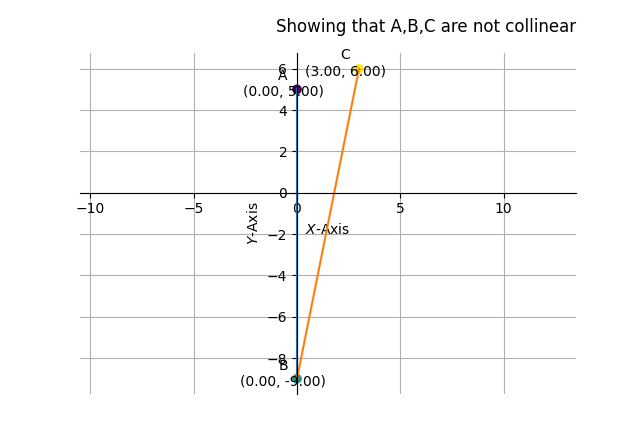
\includegraphics[width=0.7\linewidth]{figs/fig1.png}
       \caption{}
       \label{graph}
    \end{figure}



\end{document}  







